\documentclass[a4paper,12pt]{report}

\usepackage[utf8]{inputenc}
\usepackage[T1]{fontenc}
\usepackage[french]{babel} % If you write in French
\usepackage{xcolor,graphicx}


\usepackage{geometry}
\geometry{left=2cm, right=2cm, top=4cm, bottom=4cm}
\usepackage{titlesec}
\usepackage{lmodern}
\usepackage{array}


\usepackage[hidelinks]{hyperref} % Permet de rendre les liens cliquables sans les entourer d'un cadre coloré


\usepackage{fancyhdr} % Pour personnaliser les en-têtes et pieds de page
% Configuration des en-têtes et pieds de page
\pagestyle{fancy}
\fancyhf{} % Efface les en-têtes et pieds de page par défaut
\fancyhead[L]{\leftmark} % Affiche le nom du chapitre à gauche
\fancyfoot[R]{\thepage} % Affiche le numéro de page au centre du pied de page


\usepackage{enumitem}
% Uniquement le premier niveau
\setlist[itemize,1]{label={.}}
% Deuxième niveau avec un point gras
\setlist[itemize,2]{label={\boldmath$\cdot$}}



\usepackage{longtable} % Pour permettre aux tableaux de se répartir sur plusieurs pages


\renewcommand{\arraystretch}{1.5} % Espacement entre les lignes du tableau


\usepackage{booktabs} % Pour un meilleur rendu du tableau
\usepackage{float}
\usepackage{caption}


\usepackage{xcolor}
\usepackage{tcolorbox}
\usepackage{listings}

% Définition d'un style de terminal
\newtcbox{\terminalbox}{on line, colback=black, colframe=black, boxrule=0pt, left=3pt, right=3pt, top=2pt, bottom=2pt, boxsep=3pt, sharp corners, enhanced}


\usepackage{acronym}

\begin{document}

%-------------------------------------------------------------------+

\begin{titlepage}
	%  \pagecolor{blue!10}
	\begin{center}
		\begin{minipage}{1.5cm}
			\begin{center}
				
\includegraphics[width=3cm,height=3cm]{images/logo/logo-arcop.png}

			\end{center}
		\end{minipage}\hfill
		\begin{minipage}{12cm}
			\begin{center}
				\textbf{ Institut de Formation Aux Normes et Technologies de l'Informatique}\\[0.1cm]
				\textbf{-Sokodé-}
				% 		\textsc{\uppercase{Université Sultan Moulay Slimane}}

				% 		\uppercase{éCOLE NATIONALE DES SCIENCES APPLIQUéES KHOURIBGA}
			\end{center}
		\end{minipage}\hfill
		\begin{minipage}{1.5cm}
			\begin{center}
				
\includegraphics[width=2.3cm,height=2.5cm]{images/logo/logo-ifnti.png}
			\end{center}

		\end{minipage}
	
		\textsc{\Large }\\[1cm]
		{\large \bfseries Rapport De Stage de Fin d'\uppercase{é}tudes}\\[0.5cm]
		{\large En vue de l'obtention du diplôme}\\[0.5cm]

		{\huge \bfseries \uppercase{Licence Informatique} \\[0.5cm] }
		{\large \bfseries Filière : Génie Informatique}
		\textsc{\Large }\\[1cm]

		% Title
		\rule{\linewidth}{0.3mm} \\[0.4cm]
		{ \huge \bfseries\color{blue!70!black} Projet de développement d'une chaîne de restauration \\[0.4cm] }
		\rule{\linewidth}{0.3mm} \\[1cm]

		{\large \bfseries Effectué à : {Sirius Digital} du  1er Aoùt 2024 au 1er Février 2025 }\\[1cm]
		% \includegraphics[width=0.3\textwidth]{logo-isae-supaero}\\[1cm]
		% Author and supervisor
		\noindent
		\begin{minipage}{0.4\textwidth}
			\begin{flushleft} \large
				\emph{\color{black}Réalisé par :}\\
				M.~\textsc{KOUTEMA} Ditoma \\
			\end{flushleft}
		\end{minipage}%
		\begin{minipage}{0.5\textwidth}
			\begin{flushright} \large
				\emph{\color{black}Encadré par:} \\
				
				M. \textsc{KPABOU} Isidore \\
			\end{flushright}
		\end{minipage}\\[1cm]

	

		% \vfill

		% Bottom of the page
		{\large \color{black}{Année universitaire}\\ \color{black}2023/2024}

	\end{center}
\end{titlepage}

%-------------------------------------------------------------------+
\pagenumbering{Roman}
%-------------------------------------------------------------------+

\chapter*{Remerciements}
\addcontentsline{toc}{chapter}{Remerciements}
\thispagestyle{empty}

En premier lieu, je tiens à exprimer ma profonde gratitude envers Dieu, le Tout-Puissant, pour m’avoir accordé la force, le courage et la persévérance nécessaires à la réalisation de ce travail.\\

Je souhaite adresser mes remerciements les plus sincères à \textbf{M. KPABOU Isidor} et,\textbf{M. NGADEAU Hassan} mes tuteurs de stage, pour leurs accompagnement exceptionnel, leurs suivi rigoureux et les précieux conseils qu’il m’a prodigués tout au long de cette expérience. Son professionnalisme et sa bienveillance ont été des atouts majeurs dans l’accomplissement de ce projet.\\

Je tiens également à remercier chaleureusement \textbf{M. OURO BODI}, Directeur général (\ac{Sirius Digital}), pour m’avoir offert l’opportunité d’intégrer son institution et pour son soutien constant durant cette période.\\


Je tiens à témoigner ma reconnaissance aux membres du jury pour l’honneur qu’ils me font en acceptant d’évaluer ce travail. Leur expertise et leurs retours seront d’une grande valeur pour moi.\\

Enfin, je souhaite exprimer ma gratitude à l’ensemble de l’équipe pédagogique et administrative de l’\textbf{\ac{IFNTI}} pour leur engagement et leur dévouement à offrir une formation de qualité, ainsi que pour leur soutien tout au long de ce parcours académique.\\

À toutes les personnes qui, de près ou de loin, ont contribué à la réalisation de ce travail, je témoigne ici ma plus profonde reconnaissance. Leur soutien a été un pilier essentiel dans l’aboutissement de ce projet.

\clearpage
%-------------------------------------------------------------------+
\chapter*{Annexe}
\addcontentsline{toc}{chapter}{Annexe}
\thispagestyle{empty}
\clearpage
%-------------------------------------------------------------------+

\tableofcontents
\thispagestyle{empty}
\clearpage

\listoffigures
\thispagestyle{empty}
\clearpage

\listoftables
\thispagestyle{empty}
\clearpage

%-------------------------------------------------------------------+
\chapter*{Sigles, Acronymes et Abréviations}
\addcontentsline{toc}{chapter}{Sigles, Acronymes et Abréviations}

\begin{acronym}[SIRIUS DIGITAL] % Ajuste la largeur selon le plus long acronyme
  \acro{SIRIUS DIGITAL}{Autorité de Régulation de la Commande Publique}
  \acro{IFNTI}{Institut de Formation aux Normes et Technologies de l'Informatique}

  %=============================================================
  \acro{API}{Application Programming Interface}
  \acro{CSS}{Cascading Style Sheets}
  \acro{DBMS}{Database Management System}
  \acro{HTML}{HyperText Markup Language}
  \acro{JS}{JavaScript}
  \acro{JSON}{JavaScript Object Notation}
  \acro{PHP}{Hypertext Preprocessor}
  \acro{SQL}{Structured Query Language}
\end{acronym}
\clearpage

%-------------------------------------------------------------------+
%-------------------------------------------------------------------+
\pagenumbering{arabic}

\chapter*{Introduction Générale}
\addcontentsline{toc}{chapter}{Introduction Générale}
\thispagestyle{empty}
\clearpage
\section*{contexte}
\thispagestyle{empty}


Dans le cadre de leur formation, les étudiants en troisième année de l'Institut de Formation aux Normes et Technologies de l'Informatique doivent effectuer un stage de fin d’études au sein d’une organisation avant l’obtention de leur diplôme. Cette immersion professionnelle vise à leur permettre d’acquérir des compétences pratiques et à mieux appréhender le fonctionnement du monde du travail.\\

C’est dans cette perspective que le stage a été réalisé au sein de SIRIUS DIGITAL. Sirius Digital est une startup créé en 2022 et a pour but de répondre aux en jeux grandissant des nouvelles technologies en proposant des solutions à travers la conception des applications web et mobile.

Le présent rapport a pour objectif de présenter les différentes missions effectuées au sein de Sirius Digital, ainsi que les réalisations techniques développées au cours du stage. Il met en lumière les compétences acquises et les défis rencontrés, tout en illustrant l’apport de cette expérience dans le cadre de la formation académique.\\

\section*{Objectifs}

L’objectif principal de ce stage de fin d’études est de permettre à l’étudiant de mettre en pratique ce qu’il aura acquis tout au long de sa formation en licence d’informatique des organisations à l’\ac{IFNTI}, que ce soit en termes de compétences techniques comme de compétences humaines et professionnelles. L’étudiant devra être capable de s’adapter rapidement aux besoins de l’organisation afin de s’intégrer aux projets sur lesquels il travaillera. La prise en compte des démarches qualités et des méthodes associées au sein de l’organisation est primordiale. Enfin, ce stage doit permettre à l’étudiant d’acquérir une certaine autonomie technique.\\
Tout au long du stage, l’étudiant doit être accompagné d’un maitre de stage ayant entre autres pour role de l’accompagner dans son intégration au fonctionnement de l’organisation, mais aussi de le suivre en se rendant disponible.
%-------------------------------------------------------------------+
\chapter{Présentation de l'organisme d'acceuil Sirius Digital}
\clearpage
\section{Historique de Sirius Digital}

\subsection{Historique}

Fondée en 2022 par OURO BODI, Sirius Digital est une startup informatique basée à Lomé, dans le quartier de Kegué, en face du complexe scolaire Dino Golo. Dès ses débuts, l’entreprise s’est donnée pour mission de concevoir des solutions numériques innovantes répondant aux défis technologiques des entreprises, qu'elles soient petites ou grandes.

Face à l'\ac{essor} rapide des nouvelles technologies et à l’évolution croissante des besoins dans tous les secteurs, Sirius Digital s’impose progressivement comme un acteur clé dans le développement d’applications web et mobiles. Grâce à une approche axée sur l’innovation et la qualité, la startup accompagne les entreprises dans leur transformation digitale, leur offrant des outils performants et adaptés à leurs réalités.

Aujourd’hui, Sirius Digital continue d’évoluer en mettant la technologie au service du développement, avec pour ambition de devenir une référence incontournable dans le domaine des solutions numériques en Afrique et au-delà.


\begin{itemize}
    \item \textbf{Adresse :} Kegué, Lomé-TOGO, 16BP:20
    \item \textbf{Téléphone :} (+228) 91 09 16 56 / 22 61 78 84
    \item \textbf{E-mail :} \href{mailto:siriusdigital@app-siriusdigital.com}{siriusdigital@app-siriusdigital.com}
    \item \textbf{Site web :} \href{https://app-siriusdigital.com}{app-siriusdigital.com}
\end{itemize}



\section{Les organes de SIRIUS DIGITAL}
\begin{center}
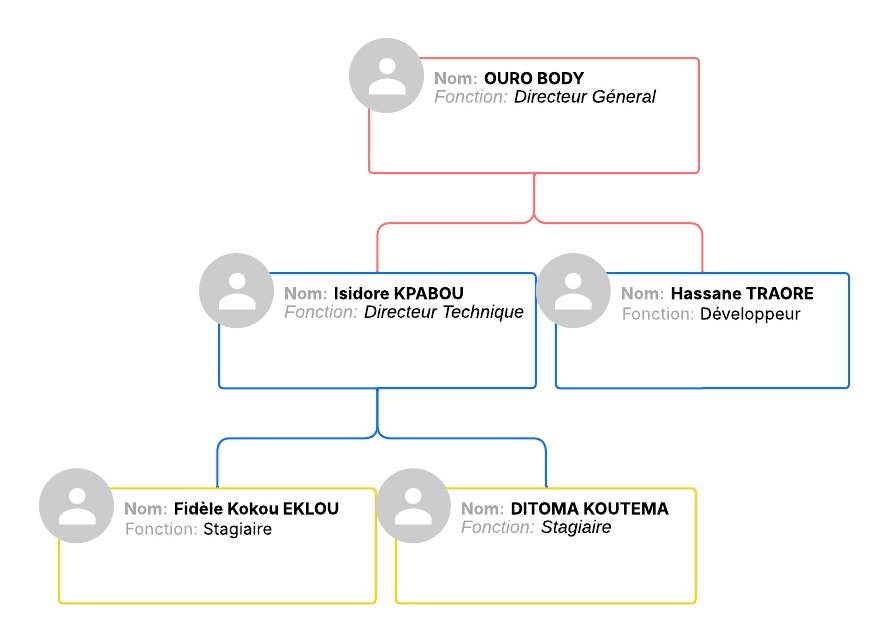
\includegraphics[scale=0.5]{images/logo/foc.png}
\end{center}




\clearpage
%-------------------------------------------------------------------+
\chapter{Déroulement du stage}
\clearpage


\section{Prise de fonction}
J'avais commencé officiellement le stage le 1er Août 2024 dans les locaux de la Société Sirius Digital. J'ai bien été accueillis dans le cadre du stage. 
Le stage commence tous les jours de 7h à 12h et de 14h à 17h de lundi à Vendredi marquée par une pose de 12h à 14h ou l'on es libre de ses actions.
L'entreprise m'a été présenté par un des membres de l'équipe déjà en place suivit d'une explication de DG qui, avait bien compris ma mission au sein de l'entreprise et m'expliquer les choses étapes par étapes pour l'avancement du projet.


\begin{itemize}
    \item Découvert l'environnement de travail et les outils utilisés.
    \item Échangé avec les membres de l'équipe et le DG pour mieux comprendre les besoins et le cadre du stage.

\end{itemize}
\section{Tâches effectuées}
Pendant ce stage, j'ai eu à effectuer plusieurs tâches notamment
\begin{itemize}
    \item Modélisation des différents diagrammes
    \item Développement Web
    \item Rédaction du support technique
    \item Rédaction du manuel d'utilisation    
\end{itemize} 


\subsubsection{Illustration}
\begin{figure}[H]
    \centering
    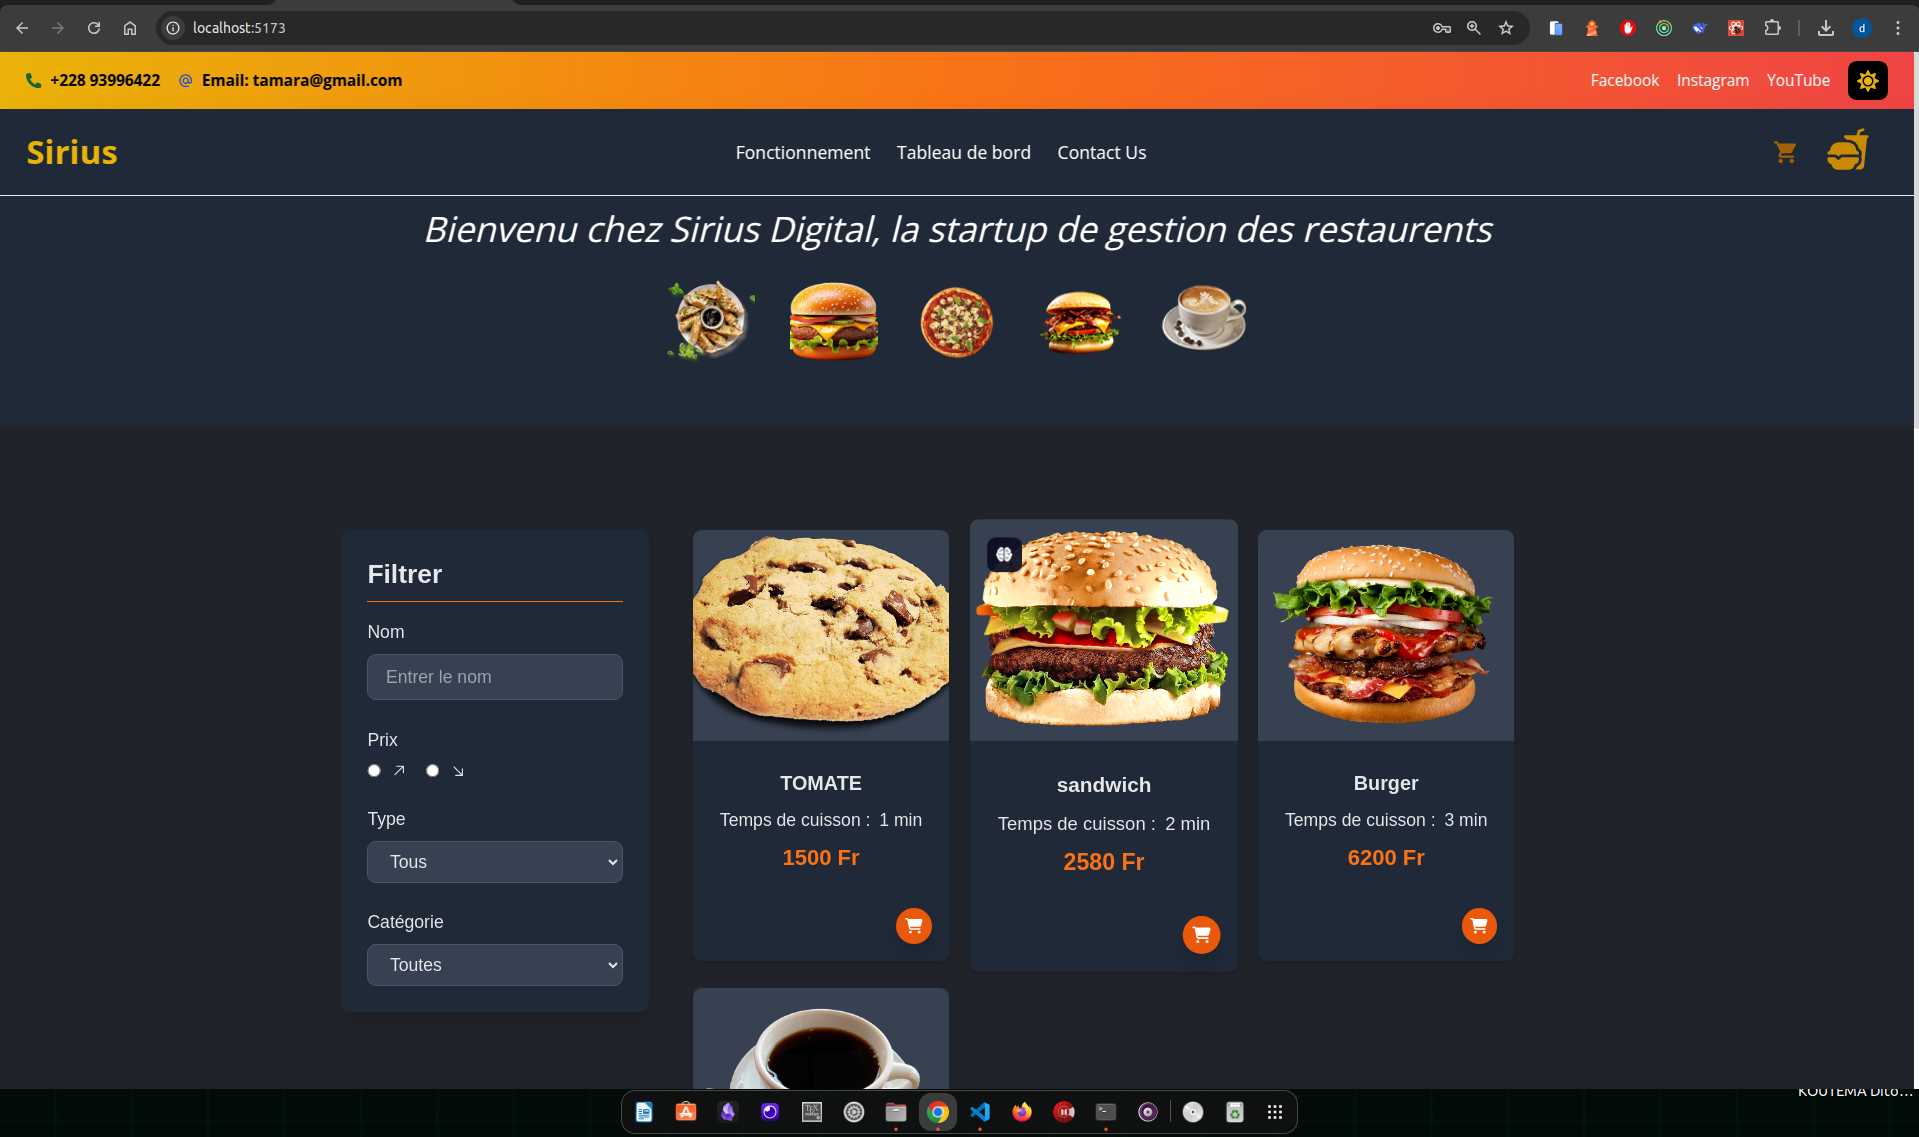
\includegraphics[width=0.8\textwidth]{images/passe/home.png}
    \caption{Page d'accueil de la \ac{PASSE}}
    \label{fig:page-accueil_pass}
\end{figure}

\begin{figure}[H]
    \centering
    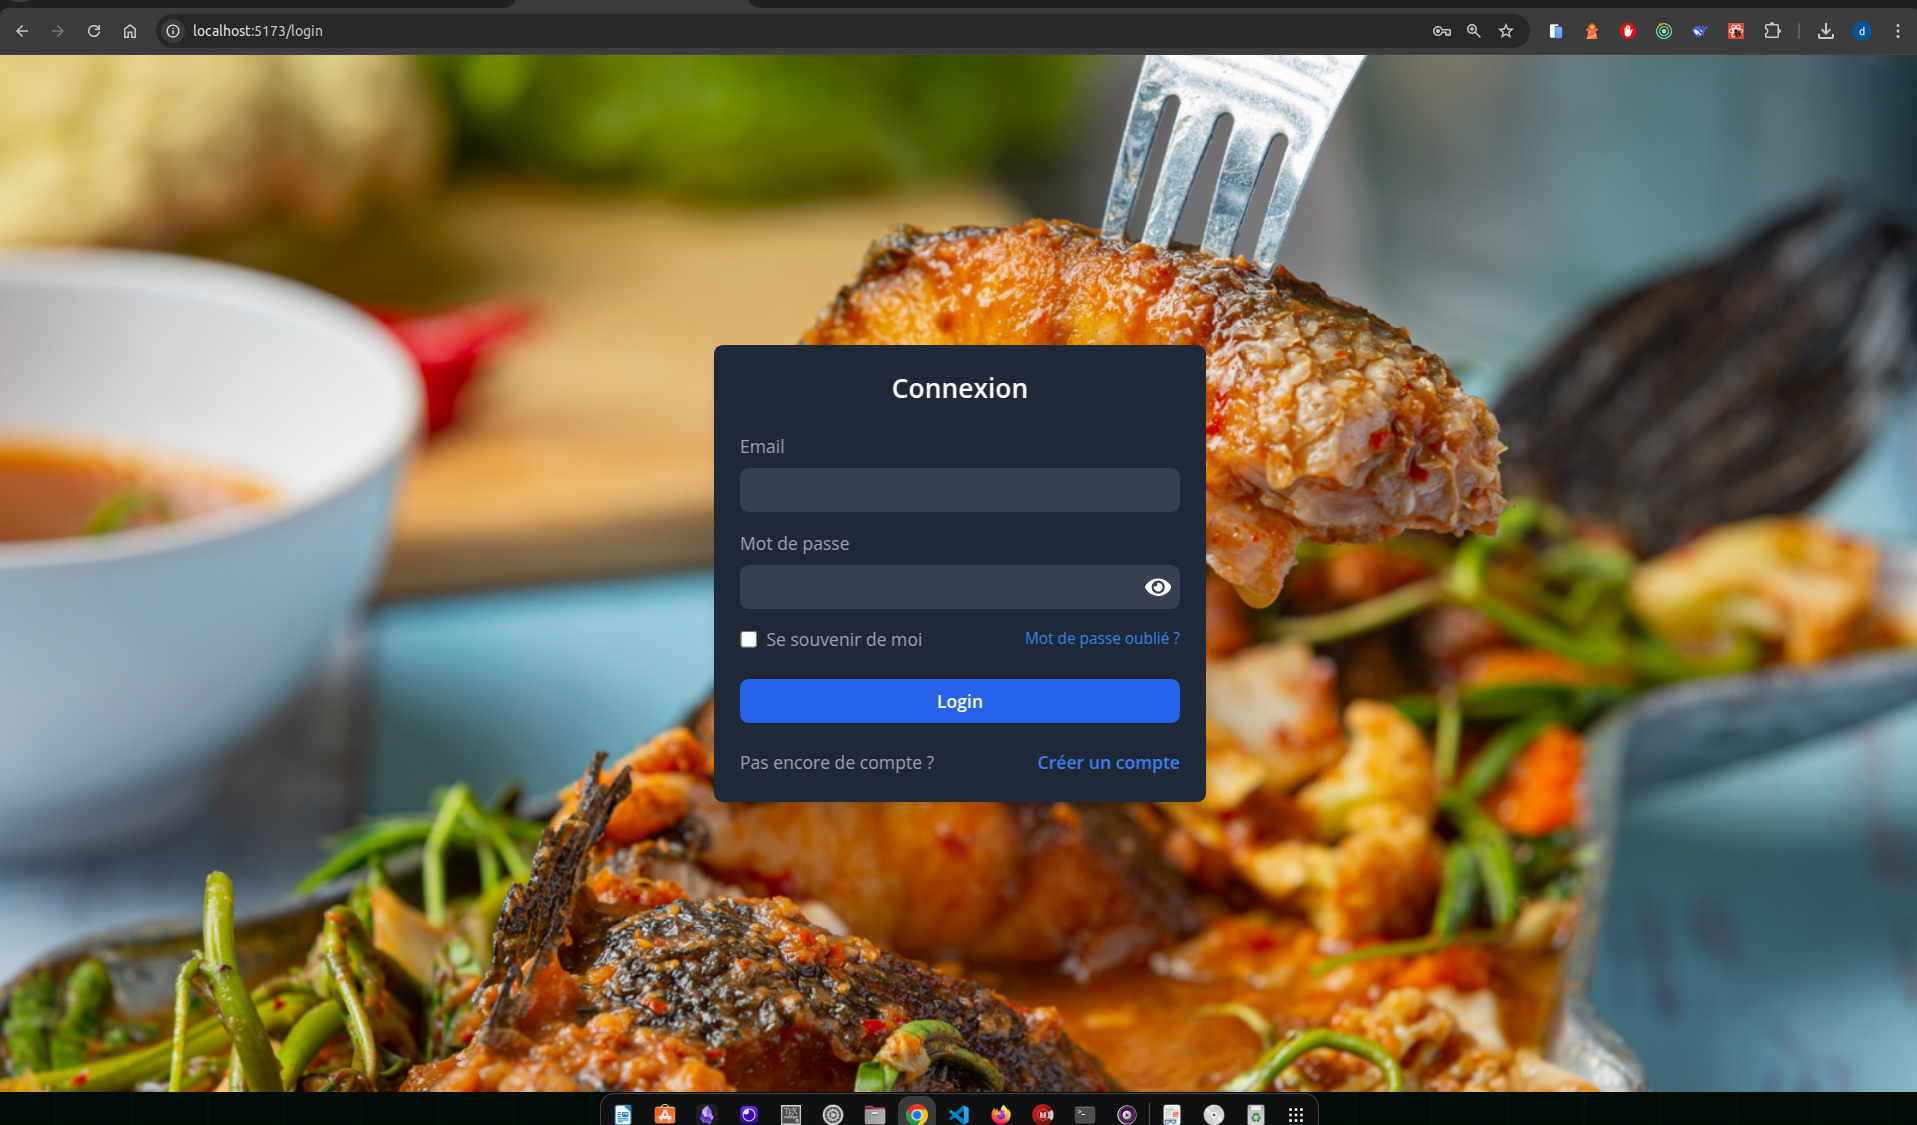
\includegraphics[width=0.8\textwidth]{images/passe/login.png}
    \caption{Interface de connexion de la \ac{PASSE}}
    \label{fig:interface-login_pass}
\end{figure}

\begin{figure}[H]
    \centering
    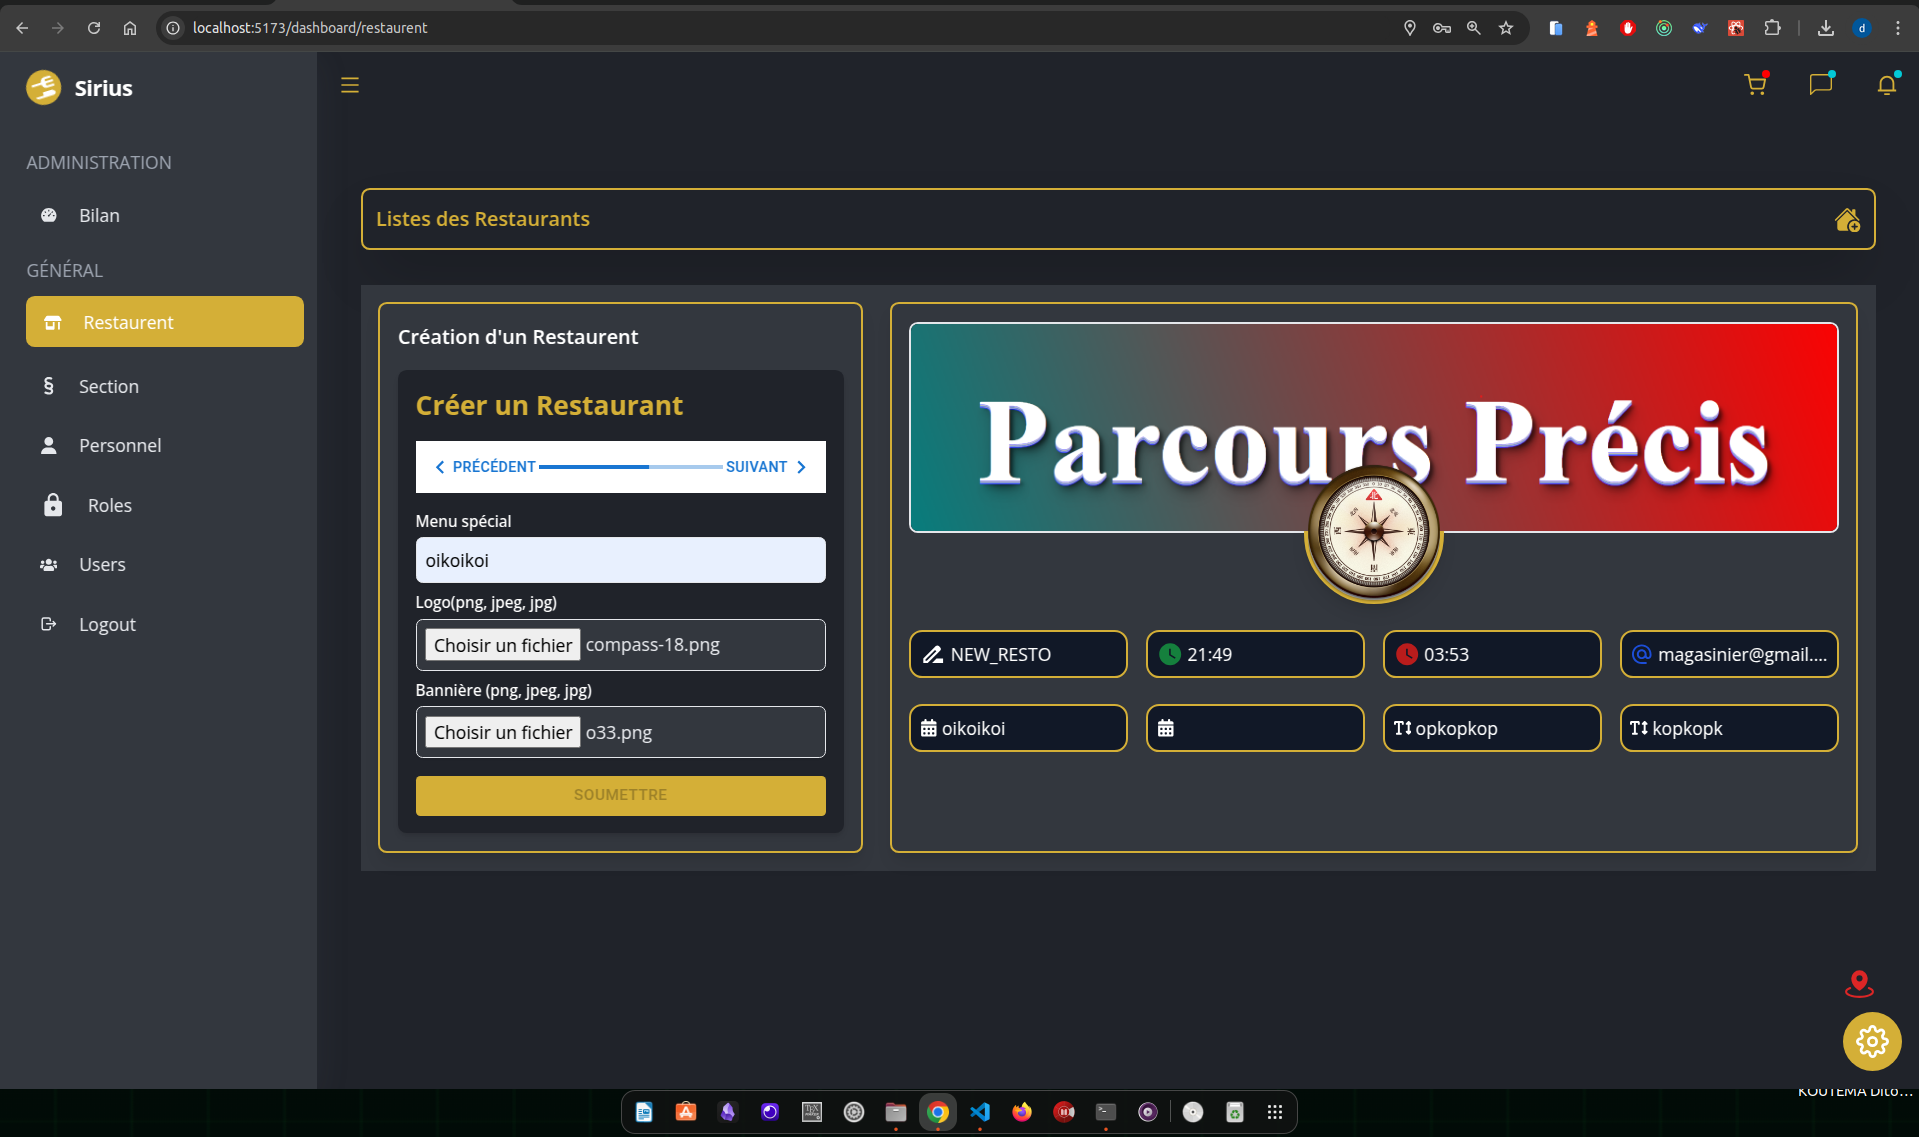
\includegraphics[width=0.8\textwidth]{images/passe/dash.png}
    \caption{Interface de connexion de la \ac{PASSE}}
    \label{fig:interface-login_pass}
\end{figure}








\subsection{Assistance technique générale}
En complément des missions spécifiques, un support technique global a été assuré au sein de l’organisation :
\begin{itemize}
    \item Dépannage et maintenance des outils informatiques utilisés par le personnel.
    \item Configuration et optimisation des postes de travail selon les besoins des employés.
    \item Sensibilisation aux bonnes pratiques pour garantir la pérennité des équipements et la sécurité des données.
\end{itemize}
\section{Remarques et suggestions}
\section{Bilan et conclusion}
Cette expérience a permis de mieux appréhender les enjeux liés à la gestion d’un service informatique, alliant assistance aux utilisateurs, maintenance technique et développement d’outils numériques.

\clearpage

%-------------------------------------------------------------------+
\chapter{Expression des besoins}
\clearpage
\section{introduction}
Ce projet vise à créer une marketplace dédiée à la restauration, où chaque utilisateur aura la possibilité de lancer et de gérer son propre restaurant en ligne. Grâce à une interface intuitive, il pourra personnaliser son espace, gérer son menu, suivre les commandes en temps réel et administrer son personnel selon ses besoins.  

L’objectif est d’offrir une solution flexible et évolutive qui permettra aux restaurateurs, qu’ils soient indépendants ou en réseau, d’optimiser leur gestion et d’atteindre une clientèle plus large. Cette plateforme mettra également à disposition des outils de suivi des performances, des options de paiement sécurisées et des fonctionnalités facilitant l’interaction avec les clients.  

En intégrant des fonctionnalités modernes et une expérience utilisateur fluide, cette marketplace ambitionne de révolutionner la manière dont les restaurants gèrent leurs activités en ligne.  


\subsection{Spécifications techniques}

\subsubsection{Langages et Technologies}
\begin{itemize}
    \item \textbf{Framework :} Laravel (passport) pour une gestion efficace de la logique serveur et du backend (developpement d'api).
    \item \textbf{Base de données :} MySQL ou PostgreSQL pour la gestion des données avec Eloquent ORM.
    \item \textbf{Frontend :} React js pour une interface utilisateur dynamique et fluide.

\end{itemize}


\subsubsection{Sécurité}
\begin{itemize}
    \item Chiffrement des données sensibles.
    \item Gestion des accès par rôles.
\end{itemize}

\subsubsection{Hébergement}
\begin{itemize}
    \item Déploiement sur les serveurs internes de Sirius Digital.
\end{itemize}
\subsection{Exigences non fonctionnelles}



\subsubsection{Utilisabilité}
\begin{itemize}
    \item L'interface utilisateur doit être intuitive et facile à utiliser, avec une courbe d'apprentissage minimale.
    \item Une documentation utilisateur complète doit être fournie, incluant des guides et des tutoriels.
\end{itemize}

\subsubsection{Compatibilité}
\begin{itemize}
    \item \textbf{Navigateurs :} Le logiciel doit être compatible avec les dernières versions de Chrome, Firefox, Safari, et Edge.
    \item \textbf{Mobile :} L'application web doit être responsive et accessible depuis les navigateurs mobiles.
\end{itemize}

\subsubsection{Scalabilité}
Le logiciel doit pouvoir gérer un nombre croissant d'utilisateurs et de données sans dégradation des performances.


\subsubsection{Nom du logicièl}
Le logiciel portera donc le nom S


\section{Définition des acteurs système}
Le logiciel est destiné à tous les utilisateurs souhaitant créer et gérer leur propre restaurant.
\begin{itemize}
    \item Client
    \item Serveur 
    \item Caissier
    \item ChefSection
    \item DG 
\end{itemize}
\subsection{Client}
L'utilisateur \textbf{Client} est simplement un utilisateur quelconque qui peut utiliser le logiciel pour commander un plat.
De même après s'être inscrit, a aussi le choix de créer et gérer son propre restaurent.
\subsection{Serveur}
Le \textbf{Serveur} est un personnel appartenant à un restaurent donné qui inter-agit avec le système pour passer des commandes en interne pour les client sur place.

\subsection{Caissier }
Le \textbf{Casier} est un personnel appartenant à un restaurent donné qui enregistrer les factures et gères beaucoup d'autres choses.

\subsection{ChefSection}
Le \textbf{DG} est un personnel appartenant à un restaurent donné, il est en quelque sorte le sous directeur du restaurent auquel il appartient. De ce fait il à beaucoup de responsabilité.

\subsection{DG}
Le \textbf{DG} est le propriétaire du restaurent, de ce fait il a le contrôle absolu du système de gestion du restaurent à travers l'application.

\section{D\'efinition des cas d'utilisation}

Un diagramme de cas d'utilisation est une représentation graphique des interactions entre les acteurs d'un système et ses fonctionnalités. Il permet d'identifier et de structurer les besoins fonctionnels du logiciel en décrivant les actions réalisées par chaque acteur. Ce type de diagramme est particulièrement utile pour comprendre les interactions des utilisateurs avec le système et pour définir clairement les responsabilités de chaque acteur.

Dans ce contexte, nous définissons les cas d'utilisation pour chaque fonctionnalités énoncés précédemment.
\subsection{Listes des cas d'utilisation}
\subsubsection{Description de chaque fonctionalité}
Cette application en son sein regroupe beaucoup de fonctionnalités telles que :
\subsubsection{Gestion de restaurent}
\begin{itemize}
    \item \textbf{Demande de congé :} L'employé peut demander un congé en ligne, en précisant la date, la durée, et le motif.
    \item \textbf{Annulation de la demande de congé :} L'employé peut annuler sa demande de congé en ligne tant que son supérieur hiérarchique n'a pas encore effectué d'action.
    \item \textbf{approbation du supérieur :} Le supérieur hiérarchique peut valider ou refuser la demande de congé de l'employé.
    \item \textbf{Approbation du GRH :} Le GRH peut valider ou refuser la demande de congé après approbation du supérieur.
    \item \textbf{Validation du DG :} Le DG peut valider ou refuser la demande de congé après approbation du GRH.
\end{itemize}


\subsubsection{Diagramme de cas d'utilisation par acteur du système}
\begin{figure}[H]
    \centering
    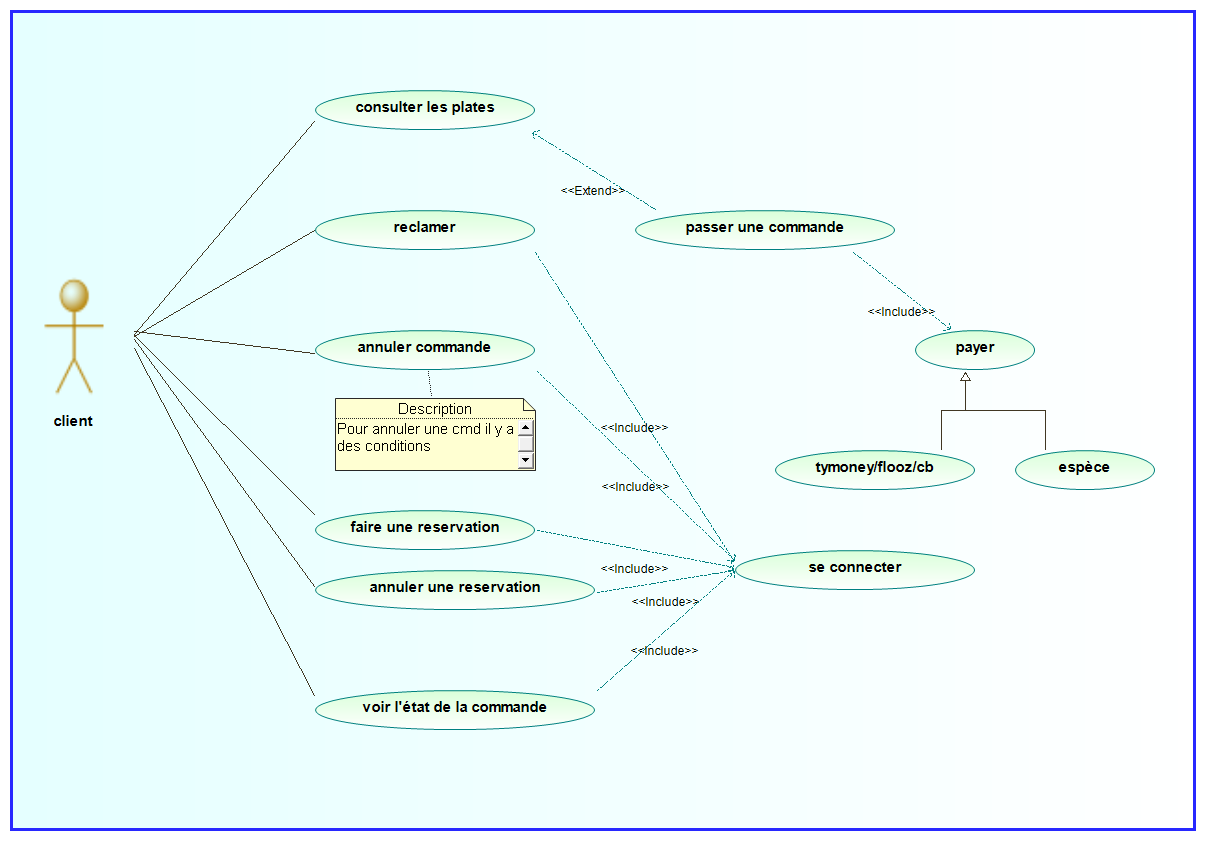
\includegraphics[width=0.8\textwidth]{images/diagrammes/use-cases/client.png}
    \caption{Diagramme de cas d'utilisation Gestion des Congés et Absences}
    \label{fig:use_case_gestion_conges}

\end{figure}


\begin{figure}[H]
    \centering
    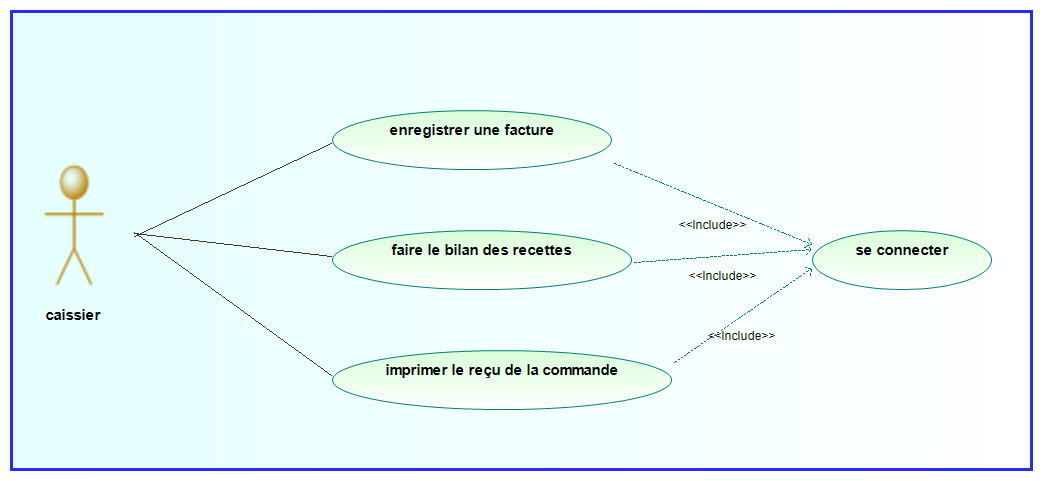
\includegraphics[width=0.8\textwidth]{images/diagrammes/use-cases/caissier.png}
    \caption{Diagramme de cas d'utilisation Gestion des Congés et Absences}
    \label{fig:use_case_gestion_conges}

\end{figure}


\begin{figure}[H]
    \centering
    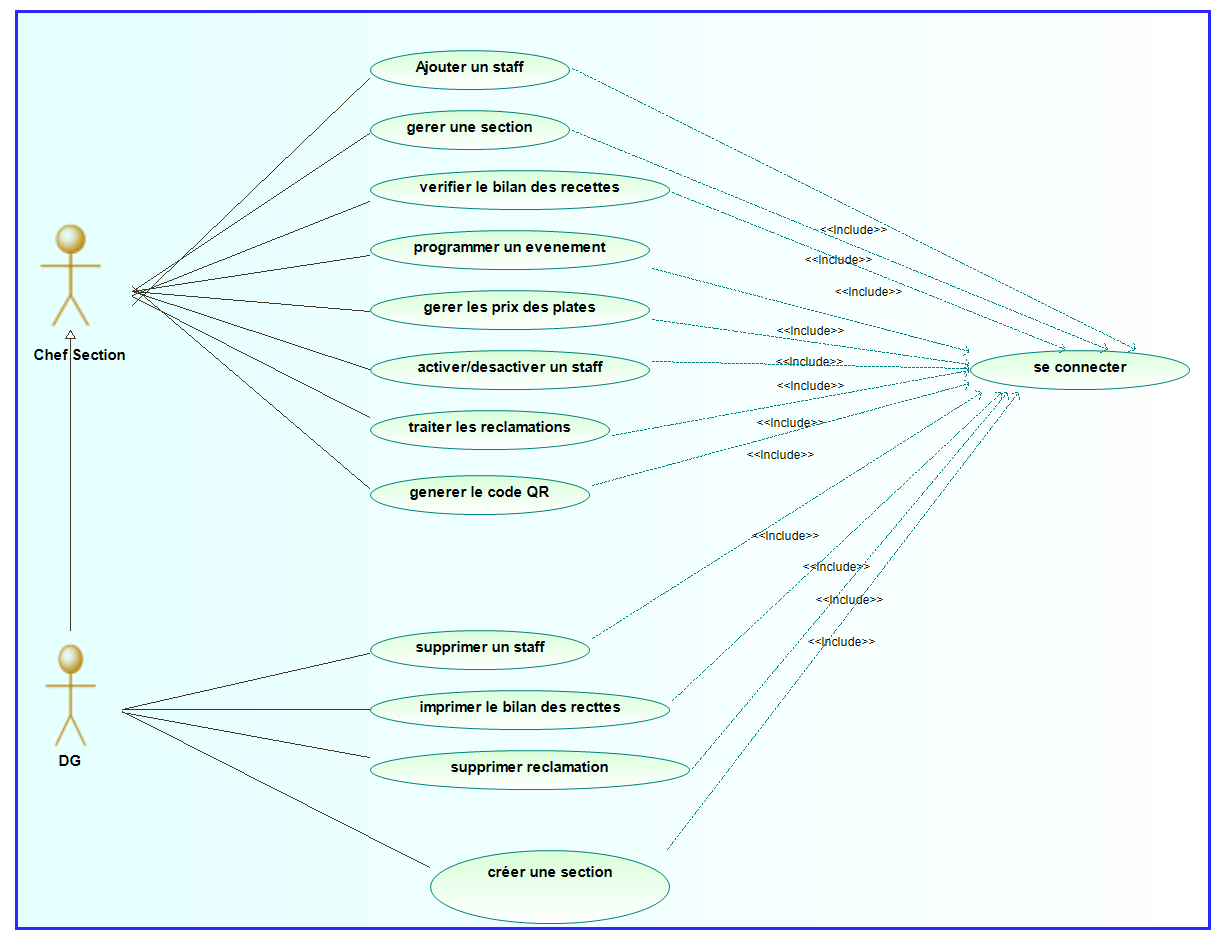
\includegraphics[width=0.8\textwidth]{images/diagrammes/use-cases/DG.png}
    \caption{Diagramme de cas d'utilisation Gestion des Congés et Absences}
    \label{fig:use_case_gestion_conges}

\end{figure}


\subsection{Gestion des dossiers}
\subsubsection{Description de la fonctionnalité}
La gestion des dossiers permet aux employés de consulter leur dossier personnel en ligne, de télécharger des bulletins de paie, et de demander des documents administratifs.
\subsubsection{Description des cas d'utilisation}
\begin{itemize}
    \item \textbf{Consultation du dossier personnel :} L'employé peut consulter son dossier personnel en ligne, contenant ses congés, absences, formations, et évaluations.
    \item \textbf{Téléchargement des bulletins de paie :} L'employé peut télécharger ses bulletins de paie depuis l'application.
    \item \textbf{Demande de documents administratifs :} L'employé peut demander des documents administratifs en ligne, tels que des attestations de travail, des certificats de travail.
\end{itemize}


\section{Conclusion}
Ce cahier des charges définit les fonctionnalités et les exigences techniques d'un logiciel de gestion des \ac{RH} performant et sécurisé pour l'\ac{ARCOP}. Le logiciel, nommé \textbf{OptiHR}, répondra aux besoins spécifiques du GRH et des employés, en facilitant la gestion des congés, des formations, et des évaluations, d'éditer les bulletins de paie tout en étant évolutif et intégrable aux systèmes existants. La prochaine étape consistera à concevoir l'architecture du système et à élaborer les diagrammes UML pour modéliser les interactions entre les différents modules.
\clearpage

%-------------------------------------------------------------------+
\chapter{Phase de réalisation du projet}
\clearpage

\section{Introduction}
Dans le cycle de développement d’un projet, la conception joue un rôle fondamental. Elle sert à établir l’architecture globale, à définir les principaux composants et à organiser les interactions entre les modules du système. Cette étape implique aussi l’identification des acteurs du système, qu’il s’agisse des utilisateurs ou des entités avec lesquelles il interagit, afin d’adapter les fonctionnalités aux besoins concrets. Une conception bien pensée assure une organisation efficace du projet, tout en simplifiant sa mise en œuvre et sa maintenance.

\section{Objectifs}
Les objectifs de la phase de conception sont les suivants :
\begin{itemize}
    \item Identifier et structurer les différents composants du système.
    \item Définir l'architecture logicielle en fonction des besoins du projet.
    \item Spécifier les interactions entre les modules pour assurer une cohérence
          globale.
    \item Concevoir les diagrammes UML, y compris les diagrammes de classes et de
          processus, afin de modéliser clairement la structure et le fonctionnement du
          système.
    \item Optimiser la conception en tenant compte des performances et de l'évolutivité.
    \item Assurer la conformité aux standards et aux bonnes pratiques du développement
          logiciel.
\end{itemize}

\section{Modélisation et diagrammes}

\subsection{Dictionnaire de données}
Le dictionnaire de données décrit en détail les attributs des entités de la
base de données, y compris leurs types, leurs rôles et leurs relations. Il
permet d'assurer la cohérence et la structuration correcte des informations
stockées.

\renewcommand{\arraystretch}{1.3} % Améliore l'espacement du tableau

\begin{longtable}{|p{3.5cm}|p{3.5cm}|p{3cm}|p{5cm}|}
    \hline
    \textbf{Nom de la table} & \textbf{Nom de l'attribut} & \textbf{Type de données}    & \textbf{Description} \\
    \hline
    \endfirsthead

    \hline
    \textbf{Nom de la table} & \textbf{Nom de l'attribut} & \textbf{Type de données}    & \textbf{Description} \\
    \hline
    \endhead

    % User
    \hline
    User                     & username                   & string                      & Nom d'utilisateur    \\
    \hline
    User                     & password                   & string                      & Mot de passe         \\
    \hline
    User                     & active                     & string                      & Statut actif/inactif \\
    \hline

    % Role
    Role                     & name                       & string                      & Nom du rôle          \\ \hline

    % Permission
    Permission               & name                       & string                      & Nom de la permission \\ \hline

    % Employee
    Employee                 & first\_name                & string                      & Prénom de l'employé  \\ \hline Employee &
    last\_name               & string                     & Nom de famille de l'employé                        \\ \hline Employee &
    phone\_number            & string                     & Numéro de téléphone                                \\ \hline Employee & email                             &
    string                   & Adresse email                                                                   \\ \hline Employee & address1 & string & Adresse
    principale                                                                                                 \\ \hline Employee & address2 & string & Adresse secondaire \\
    \hline Employee          & city                       & string                      & Ville                \\ \hline Employee & country & string &
    Pays                                                                                                       \\ \hline Employee & state & string & Région ou état \\ \hline Employee &
    bank\_name               & string                     & Nom de la banque                                   \\ \hline Employee & rib & string &
    Relevé d'identité bancaire                                                                                 \\ \hline

    % Department
    Department               & name                       & string                      & Nom du département   \\ \hline

    % File
    File                     & name                       & string                      & Nom du fichier       \\ \hline File & url & string & URL du
    fichier                                                                                                    \\ \hline File & mime\_type & string & Type MIME \\ \hline File & path
                             & string                     & Chemin d'accès                                     \\ \hline File & upload\_date & string & Date
    d'upload                                                                                                   \\ \hline

    % Duty
    Duty                     & duration                   & string                      & Durée de la mission  \\ \hline Duty & begin\_date                       &
    string                   & Date de début                                                                   \\ \hline Duty & type & string & Type de mission \\
    \hline Duty              & etat                       & string                      & État de la mission   \\ \hline

    % Job
    Job                      & title                      & string                      & Intitulé du poste    \\ \hline

    % Absence
    Absence                  & day\_requested             & string                      & Jour demandé         \\ \hline Absence &
    start\_date              & string                     & Date de début                                      \\ \hline Absence & end\_date & string &
    Date de fin                                                                                                \\ \hline Absence & address & string & Adresse \\ \hline Absence        &
    date\_of\_application    & string                     & Date de la demande                                 \\ \hline Absence & status
                             & string                     & Statut de l'absence                                \\ \hline Absence & date\_of\_approval                    & string
                             & Date d'approbation                                                              \\ \hline Absence & type\_of\_absence & string & Type
    d'absence                                                                                                  \\ \hline Absence & reasons & string & Raisons de l'absence \\ \hline
    Absence                  & proof                      & string                      & Justificatif         \\ \hline Absence & comment & string &
    Commentaire                                                                                                \\ \hline

\end{longtable}
\begin{center}  
    \captionof{table}{Tableau du dictionnaire des données} % Ajoute la légende à la liste des tableaux  
    \label{tab:table_dictionnaire_data}  
\end{center}  
\subsection{Diagramme de classes}
Le diagramme de classes permet de représenter les différentes entités du
système et leurs relations. Il offre une vision claire de la structure et
facilite la compréhension des interactions entre les objets.

\begin{figure}[H]
    \centering
    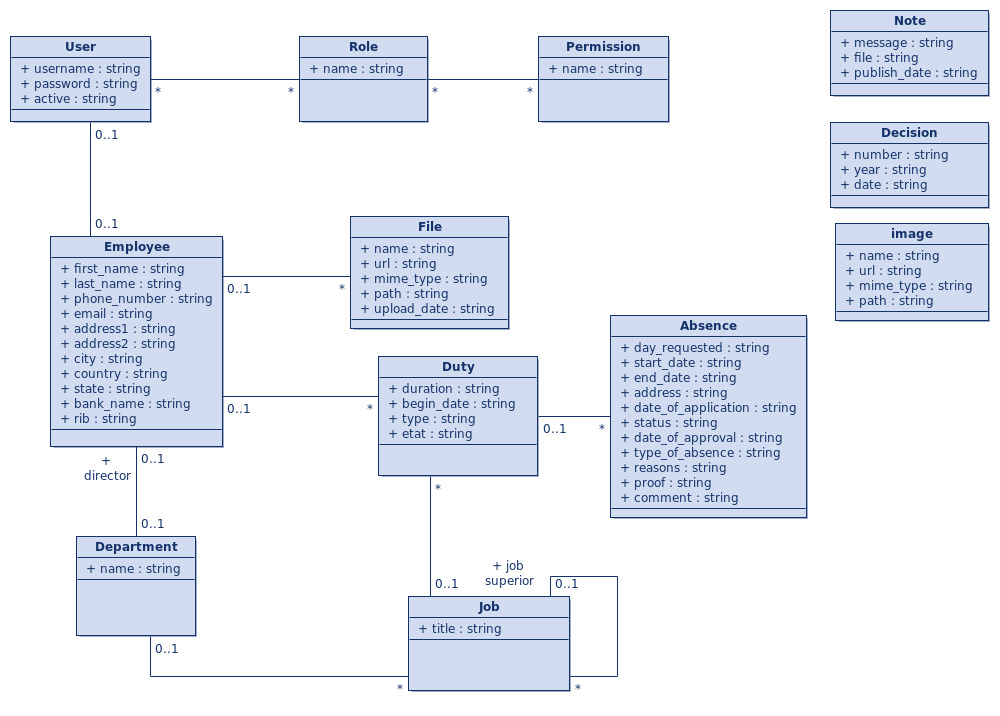
\includegraphics[width=0.8\textwidth]{images/diagrammes/class/diagramme.jpeg}
    \caption{Diagramme de classe - Gestion du projet OptiHR}
    \label{fig:class_diagramm_optiRH}
\end{figure}

\section{Description des entités et relations}

Le diagramme de classes représente un système de gestion des employés et de
leurs activités professionnelles. Voici une description des entités principales
et de leurs relations :

\subsection{Entités principales}

\subsubsection{User (Utilisateur)}
\textbf{Attributs} :
\begin{itemize}
    \item username
    \item password
    \item active
\end{itemize}
\textbf{Relations} : Un utilisateur est associé à un employé.

\subsubsection{Employee (Employé)}
\textbf{Attributs} :
\begin{itemize}
    \item first\_name
    \item last\_name
    \item phone\_number
    \item email
    \item address1
    \item address2
    \item city
    \item country
    \item state
    \item bank\_name
    \item rib
\end{itemize}
\textbf{Relations} :
\begin{itemize}
    \item Un employé peut être un directeur d'un département.
    \item Un employé appartient à un seul département.
    \item Un employé peut avoir plusieurs fichiers associés.
    \item Un employé peut être lié à plusieurs absences.
\end{itemize}

\subsubsection{Department (Département)}
\textbf{Attributs} :
\begin{itemize}
    \item name
\end{itemize}
\textbf{Relations} :
\begin{itemize}
    \item Un département peut avoir un seul directeur (Employee).
    \item Un département peut contenir plusieurs employés.
\end{itemize}

\subsubsection{Role (Rôle)}
\textbf{Attributs} :
\begin{itemize}
    \item name
\end{itemize}
\textbf{Relations} : Un utilisateur peut avoir plusieurs rôles.

\subsubsection{Permission (Permission)}
\textbf{Attributs} :
\begin{itemize}
    \item name
\end{itemize}
\textbf{Relations} : Un rôle peut avoir plusieurs permissions.

\subsubsection{File (Fichier)}
\textbf{Attributs} :
\begin{itemize}
    \item name
    \item url
    \item mime\_type
    \item path
    \item upload\_date
\end{itemize}
\textbf{Relations} : Un employé peut avoir plusieurs fichiers.

\subsubsection{Duty (Tâche/Mission)}
\textbf{Attributs} :
\begin{itemize}
    \item duration
    \item begin\_date
    \item type
    \item etat
\end{itemize}
\textbf{Relations} : Un employé peut avoir plusieurs tâches.

\subsubsection{Job (Poste)}
\textbf{Attributs} :
\begin{itemize}
    \item title
\end{itemize}
\textbf{Relations} : Un employé peut avoir un seul poste.

\subsubsection{Absence (Absence)}
\textbf{Attributs} :
\begin{itemize}
    \item day\_requested
    \item start\_date
    \item end\_date
    \item address
    \item date\_of\_application
    \item status
    \item date\_of\_approval
    \item type\_of\_absence
    \item reasons
    \item proof
    \item comment
\end{itemize}
\textbf{Relations} : Un employé peut avoir plusieurs absences.

\subsubsection{Note (Note)}
\textbf{Attributs} :
\begin{itemize}
    \item message
    \item file
    \item publish\_date
\end{itemize}

\subsubsection{Decision (Décision)}
\textbf{Attributs} :
\begin{itemize}
    \item number
    \item year
    \item date
\end{itemize}

\subsubsection{Image (Image)}
\textbf{Attributs} :
\begin{itemize}
    \item name
    \item url
    \item mime\_type
    \item path
\end{itemize}

\section{Technologies et outils}
Les outils et technologies suivants ont été utilisés pour la conception du
projet \textbf{OptiHR}. Chaque outil est accompagné d'une image et d'une
description détaillée.

\vspace{1cm} % Ajoute un espace vertical

\renewcommand{\arraystretch}{1.5} % Espacement entre les lignes du tableau

\begin{center}
    \begin{table}[h]  % Environnement table pour être listé dans la liste des tableaux
       

        \begin{tabular}{|m{4cm}|m{10cm}|}
            \hline
            \textbf{Technologie}                                 & \textbf{Description}                                                                                                                                                                             \\
            \hline

            
\includegraphics[width=3cm]{images/logo/uml.png}     & \textbf{UML} : Utilisé pour la modélisation des systèmes et la conception des structures du projet. Il permet de représenter graphiquement les différentes interactions et processus du système. \\
            \hline

            
\includegraphics[width=3cm]{images/logo/modelio.png} & \textbf{Modelio} : Outil de modélisation UML permettant de créer des diagrammes tels que les diagrammes de classes, de séquence et d'activités.                                                  \\
            \hline

        \end{tabular}
        % \centering
        \caption{Tableau des technologies et outils utilisés pour la conception} % La légende du tableau
        \label{tab:technos_conception} % Étiquette pour référence
    \end{table}
\end{center}

\section{Conclusion}
La phase de conception pose les bases essentielles du projet en structurant
l'architecture et en précisant les technologies et les modèles de données
adoptés. Une conception rigoureuse garantit un développement fluide et
efficace, tout en assurant la maintenance et l'évolutivité du système sur le
long terme.

\clearpage

%-------------------------------------------------------------------+
\chapter{Réalisation}
\clearpage
\section{Introduction}
Dans cette section, nous présentons le processus de développement et d’implémentation du système basé sur le modèle conceptuel défini précédemment. Nous détaillerons les choix technologiques adoptés, l’architecture logicielle mise en place, ainsi que les différentes étapes de développement, allant de la conception de la base de données à l’intégration des fonctionnalités essentielles.

L’implémentation suivra une approche modulaire afin de garantir la maintenabilité et l’évolutivité du système. Nous mettrons également en avant les bonnes pratiques de développement, telles que la structuration du code, la gestion des dépendances et l’optimisation des performances.

Enfin, nous testerons et validerons le bon fonctionnement du système à travers des scénarios réels d’utilisation, en nous assurant qu’il répond aux exigences fonctionnelles et non fonctionnelles définies.
%===========================================================================================================

\section{Architecture du projet}
\subsection{Présentation de l'architecture globale}
% Décrire l'architecture générale (monolithe, microservices, MVC, etc.)
%===========================================================================================================

\subsection{Choix des technologies et outils}
% Expliquer les choix technologiques (Node.js, Vue.js, React.js, PostgreSQL, etc.)
% Justifier ces choix en fonction des besoins du projet

Dans cette section, nous présentons les principales technologies utilisées pour le développement du projet. Chaque technologie a été sélectionnée pour ses performances, sa robustesse et sa facilité d’intégration dans notre stack.

\vspace{1cm} % Ajoute un espace vertical


\begin{longtable}{|m{4cm}|m{10cm}|}
    \hline
    \textbf{Technologie} & \textbf{Description} \\
    \hline
    \endfirsthead

    \hline
    \textbf{Technologie} & \textbf{Description} \\
    \hline
    \endhead

    \hline
    \endfoot

    \hline
    
\includegraphics[width=3cm]{images/logo/laravel.png} & 
    \textbf{Laravel - Framework Backend} : Laravel est un framework PHP moderne basé sur l’architecture MVC (Modèle-Vue-Contrôleur). Il offre de nombreuses fonctionnalités telles que :  
    \begin{itemize}
        \item Un ORM puissant (Eloquent) pour la gestion de la base de données.
        \item Un système de migration et de seeders pour faciliter le développement.
        \item Un mécanisme de routage avancé et un middleware intégré pour la gestion des requêtes HTTP.
    \end{itemize}
    Grâce à Laravel, nous avons pu structurer le projet de manière efficace et évolutive. \\
    \hline

    
\includegraphics[width=3cm]{images/logo/blade.png} & 
    \textbf{Blade - Moteur de Templating} : Blade est le moteur de templates natif de Laravel. Il permet de créer des vues dynamiques avec une syntaxe claire et fluide. Ses principales caractéristiques sont :
    \begin{itemize}
        \item Une syntaxe simplifiée pour l'affichage des données et les structures de contrôle (`@if`, `@foreach`, etc.).
        \item La possibilité d’étendre des layouts grâce à l’héritage de templates.
        \item Une mise en cache automatique pour améliorer les performances.
    \end{itemize}\\
    \hline

    
\includegraphics[width=3cm]{images/logo/postgresql.png} & 
    \textbf{PostgreSQL - Base de Données Relationnelle} : PostgreSQL est un système de gestion de base de données relationnelle open-source reconnu pour sa stabilité et ses performances. Il a été choisi pour :  
    \begin{itemize}
        \item Son support avancé des types de données et des transactions ACID.
        \item Sa capacité à gérer de gros volumes de données efficacement.
        \item Son intégration facile avec Laravel via l'ORM Eloquent.
    \end{itemize}\\
    \hline

    
\includegraphics[width=3cm]{images/logo/bootstrap.png} & 
    \textbf{Bootstrap - Framework CSS} : Bootstrap est un framework CSS populaire utilisé pour concevoir une interface utilisateur réactive et attrayante. Il nous a permis de :  
    \begin{itemize}
        \item Utiliser un système de grille pour une mise en page responsive.
        \item Accélérer le développement avec des composants préconçus (modals, boutons, alertes, etc.).
        \item Assurer une compatibilité avec tous les navigateurs modernes.
    \end{itemize}\\
    \hline

    
\includegraphics[width=3cm]{images/logo/javascript.png} & 
    \textbf{JavaScript - Langage de Programmation Frontend} : JavaScript est un langage de programmation utilisé pour ajouter des interactions dynamiques à l'interface utilisateur. Il a été employé pour :  
    \begin{itemize}
        \item Gérer les interactions utilisateur (événements, animations).
        \item Améliorer l'expérience avec des requêtes asynchrones (AJAX, Fetch API).
        \item Dynamiser le rendu des composants sans recharger la page.
    \end{itemize}\\
    \hline

    
\includegraphics[width=3cm]{images/logo/git.png}  
    
\includegraphics[width=3cm]{images/logo/github.png} & 
    \textbf{Git et GitHub - Outils de Gestion de Version} : Pour la gestion du code source, nous avons utilisé **Git** et **GitHub** :  
    \begin{itemize}
        \item **Git** permet de suivre l'évolution du projet grâce à un système de versionnement performant.
        \item **GitHub** facilite la collaboration et l’hébergement du code en ligne, avec des fonctionnalités comme les pull requests et les issues.
    \end{itemize}
    Ces outils nous ont permis de travailler efficacement en équipe et d’assurer la stabilité du code tout au long du développement.\\
    \hline

\end{longtable}
\begin{center}  
    \captionof{table}{Tableau des technologies utilisées pour la réalisation} % Ajoute la légende à la liste des tableaux  
    \label{tab:table_techs_realisation} % Permet de faire référence à ce tableau plus tard
\end{center}  
L’utilisation de ces technologies nous a permis de construire une application performante, maintenable et évolutive. Le choix de Laravel avec Blade pour le backend, PostgreSQL pour la base de données et Bootstrap avec JavaScript pour le frontend a facilité l’implémentation et l’optimisation du projet. Enfin, l’utilisation de Git et GitHub a renforcé la gestion du code et le travail collaboratif.

%===========================================================================================================
\section{Développement et implémentation}

\subsection{Mise en place de l’environnement de développement}
% Décrire la configuration initiale du projet (installation des dépendances, structuration du code)


Pour assurer un développement fluide et efficace, un environnement de travail stable et bien configuré a été mis en place sous **Ubuntu 24**. Cette section détaille les étapes suivies pour l’installation et la configuration des outils nécessaires.

\subsubsection{Prérequis}
Les outils suivants ont été utilisés :
\begin{itemize}
    \item Système d’exploitation : \textbf{Ubuntu 24}
    \item Éditeur de code : \textbf{Visual Studio Code}
    \item Serveur Web et PHP : \textbf{Apache, PHP 8.2}
    \item Base de données : \textbf{PostgreSQL}
    \item Gestionnaire de paquets : \textbf{Composer (pour PHP) et npm (pour JavaScript)}
    \item Système de versionnement : \textbf{Git et GitHub}
\end{itemize}

\subsubsection{Installation des outils}

\subsubsection*{Installation de PHP 8.2 et Apache}
Ubuntu 24 ne propose pas PHP 8.2 par défaut. Pour l’installer avec Apache :
\begin{tcolorbox}[colback=black, coltext=white, title=Installation de PHP 8.2 et Apache, fonttitle=\bfseries]
\texttt{sudo apt update \&\& sudo apt upgrade -y} \\
\texttt{sudo apt install apache2 php8.2 libapache2-mod-php8.2 php8.2-cli php8.2-mbstring php8.2-xml php8.2-curl php8.2-pgsql unzip -y}
\end{tcolorbox}

Une fois l’installation terminée, redémarrer Apache :

\begin{tcolorbox}[colback=black, coltext=white, title=Redémarrage du serveur Apache, fonttitle=\bfseries]
\texttt{sudo systemctl restart apache2}
\end{tcolorbox}

Vérifier que PHP est bien installé :

\begin{tcolorbox}[colback=black, coltext=white, title=Vérification de la version de PHP, fonttitle=\bfseries]
\texttt{php -v}
\end{tcolorbox}

\subsubsection*{Installation de Composer}
Composer est indispensable pour gérer les dépendances PHP :

\begin{tcolorbox}[colback=black, coltext=white, title=Installation de Composer, fonttitle=\bfseries]
\texttt{curl -sS https://getcomposer.org/installer | php} \\
\texttt{sudo mv composer.phar /usr/local/bin/composer} \\
\texttt{composer -V}
\end{tcolorbox}

\subsubsection{Installation et configuration de PostgreSQL}
PostgreSQL est utilisé comme base de données :

\begin{tcolorbox}[colback=black, coltext=white, title=Installation de PostgreSQL, fonttitle=\bfseries]
\texttt{sudo apt install postgresql postgresql-contrib -y}
\end{tcolorbox}

Démarrer PostgreSQL et vérifier son installation :

\begin{tcolorbox}[colback=black, coltext=white, title=Démarrage et vérification, fonttitle=\bfseries]
\texttt{sudo systemctl start postgresql} \\
\texttt{sudo systemctl enable postgresql} \\
\texttt{psql --version}
\end{tcolorbox}

\subsubsection*{Installation de Laravel}
Créer un projet Laravel :

\begin{tcolorbox}[colback=black, coltext=white, title=Création d’un projet Laravel, fonttitle=\bfseries]
\texttt{composer create-project --prefer-dist laravel/laravel:\^10.0 nom\_du\_projet}
\end{tcolorbox}

Générer la clé d’application :

\begin{tcolorbox}[colback=black, coltext=white, title=Génération de la clé d’application, fonttitle=\bfseries]
\texttt{php artisan key:generate}
\end{tcolorbox}

\subsubsection{Configuration de Git et clonage du projet}
Vérifier si Git est installé :

\begin{tcolorbox}[colback=black, coltext=white, title=Vérification de Git, fonttitle=\bfseries]
\texttt{git --version}
\end{tcolorbox}

Si Git n’est pas installé, l’ajouter avec :

\begin{tcolorbox}[colback=black, coltext=white, title=Installation de Git, fonttitle=\bfseries]
\texttt{sudo apt install git -y}
\end{tcolorbox}

Cloner le projet depuis GitHub :

\begin{tcolorbox}[colback=black, coltext=white, title=Clonage du projet, fonttitle=\bfseries]
\texttt{git clone https://github.com/utilisateur/nom\_du\_projet.git} \\
\texttt{cd nom\_du\_projet}
\end{tcolorbox}

\subsubsection{Lancement du serveur de développement}
Démarrer Laravel en mode développement :

\begin{tcolorbox}[colback=black, coltext=white, title=Lancement du serveur Laravel, fonttitle=\bfseries]
\texttt{php artisan serve}
\end{tcolorbox}

L’application est maintenant accessible à l’adresse :

\begin{tcolorbox}[colback=black, coltext=white, title=URL d’accès, fonttitle=\bfseries]
\texttt{http://127.0.0.1:8000/}
\end{tcolorbox}






\subsection{Développement des fonctionnalités principales}
% Présenter les fonctionnalités principales du projet et leur implémentation

\subsubsection{Feature 1 : [Nom de la fonctionnalité]}
% Détailler le développement d’une fonctionnalité clé

\subsubsection{Feature 2 : [Nom de la fonctionnalité]}
% Détailler une autre fonctionnalité clé

\section{Problèmes rencontrés et solutions adoptées}
\subsection{Difficultés techniques}
% Problèmes liés aux technologies utilisées, performances, compatibilité

\subsection{Optimisation et amélioration du code}
% Améliorations mises en place pour optimiser le projet

\section{Tests et validation}
\subsection{Stratégie de test}
% Présentation des tests utilisés (unitaires, intégration, end-to-end)

\subsection{Résultats des tests}
% Analyse des résultats des tests et validation du bon fonctionnement

\section{Conclusion}
% Résumer les étapes clés de la réalisation et l’impact des choix technologiques
\clearpage
%-------------------------------------------------------------------+
\chapter{Bilan}
\clearpage

\section{Introduction}
Dans ce chapitre, nous faisons le bilan du projet en revenant sur les objectifs fixés, les résultats obtenus, les compétences acquises ainsi que les perspectives d'amélioration.

\section{Retour sur les objectifs initiaux}
\subsection{Rappel des objectifs du projet}
% Décrire les objectifs de départ

\subsection{Évaluation de leur atteinte}
% Comparaison des objectifs avec les résultats obtenus

\section{Analyse des résultats obtenus}
% Expliquer les résultats concrets et les comparer aux attentes initiales

\subsection{Synthèse des résultats}
% Présenter une vue d’ensemble des réalisations

\subsection{Difficultés rencontrées et solutions adoptées}
% Détailler les problèmes survenus et les solutions mises en place

\section{Compétences acquises et développées}
\subsection{Compétences techniques}
% Technologies, outils, frameworks utilisés et maîtrisés

\subsection{Compétences organisationnelles}
% Gestion de projet, travail en équipe, méthodologies

\subsection{Compétences personnelles}
% Autonomie, prise de décision, esprit critique

\section{Limites et axes d’amélioration}
\subsection{Contraintes techniques et organisationnelles}
% Identifier les principales limites rencontrées

\subsection{Améliorations possibles et perspectives d’évolution}
% Propositions pour améliorer le projet à l’avenir

\section{Conclusion}
% Résumer les points clés et l’impact du projet sur le parcours professionnel
\clearpage

%-------------------------------------------------------------------+
\chapter{Conclusion Générale}
\clearpage

\end{document}